\documentclass[
    a4paper,
    keeplastbox,            % Prevents problems with last line in references
    hyphens,                % Allow hyphenation in \url
    nospread,               % Suppress whitespace fill for column balancing
    refpage,                % Separate references page
%     boxit,                  % Show margins (debug only)
]{jacow}

\usepackage{amsmath}


% Tricky hack to make the last line of each caption aligned.  This is ... umm ..
% perhaps not altogether necessary, but I like the result.
\newcommand{\squarecaption}[2][1]{\caption[#1]{#2\unskip\parfillskip 0pt}}

\hyphenpenalty 2000         % Tone down hyphenation


% Not a huge fan of the legacy Fraktur symbols for Re/Im
\renewcommand{\Re}{\operatorname{re}}
\renewcommand{\Im}{\operatorname{im}}

\newcommand{\R}{\mathbb{R}}

% Nice trick for .. described here: https://tex.stackexchange.com/a/304667
\newcommand{\dotdot}{\mathinner{\ldotp\ldotp}}


\begin{document}
\title{%
    Tune Computation via Model Fitting to Swept Machine Response Measurement}
\author{%
    M.G.~Abbott\thanks{michael.abbott@diamond.ac.uk},
    G.~Rehm, Diamond Light Source, UK}
\maketitle

\begin{abstract}

At Diamond Light Source we compute the horizontal and vertical tunes by fitting
a simple multi-pole resonator model to the measured electron beam frequency
response.  The transverse (and longitudinal) tune response is measured by
sweeping an excitation across the range of possible tune frequencies and
synchronously measuring the IQ response.

The multi-pole resonator model is a good fit to the measured behaviour, but the
fitting process is surprisingly challenging.  Problems include noisy
measurements, very complex beam responses in the presence of increasing
chromaticity, poor data when the beam is close to instability, and a number of
challenges with the stability of the algorithm.

The tune fitting algorithm now in use at Diamond has been developed and refined
over many years.  It is finally stable enough to work reliably throughout most
beam operating conditions.  The algorithm involves alternating peak finding and
non-linear fitting, with a fairly naive mathematical approach; the main focus is
on providing reliable results.

\end{abstract}


\section{Introduction}

The synchrotron beam has natural frequencies of oscillation in the horizontal,
vertical, and longitudinal directions: transverse ``betatron tunes'' and
longitudinal ``synchrotron tunes''.  The precise betatron tune frequencies are
of considerable interest to machine physicists, and need to be measured at
various stages during machine operation.

At Diamond Light Source the storage ring configuration has evolved into a state
where movement of the tunes (driven mainly by insertion device movements
affecting machine optics) can result in loss of beam lifetime and injection
efficiency, so it is necessary to actively measure and correct the betatron
tunes in both transverse axes.  This therefore requires a reliable measurement
of the tunes, during both machine startup conditions and normal operation.

A complicating factor when computing the tunes arises from interference between
transverse and longitudinal oscillations, depending on the chromaticity settings
of the synchrotron.  This interaction can result in significant side-lobes at
(roughly) multiples of synchrotron frequency offset either side of the main tune
measurement.  Depending on machine conditions it can become difficult to
identify the central tune frequency.  This is addressed by the process described
here, but there remain some operating conditions that can be surprisingly
difficult to interpret.

We are able to take advantage of phase and magnitude measurement to fit a
reasonably sophisticated model.


\begin{figure}[ht]
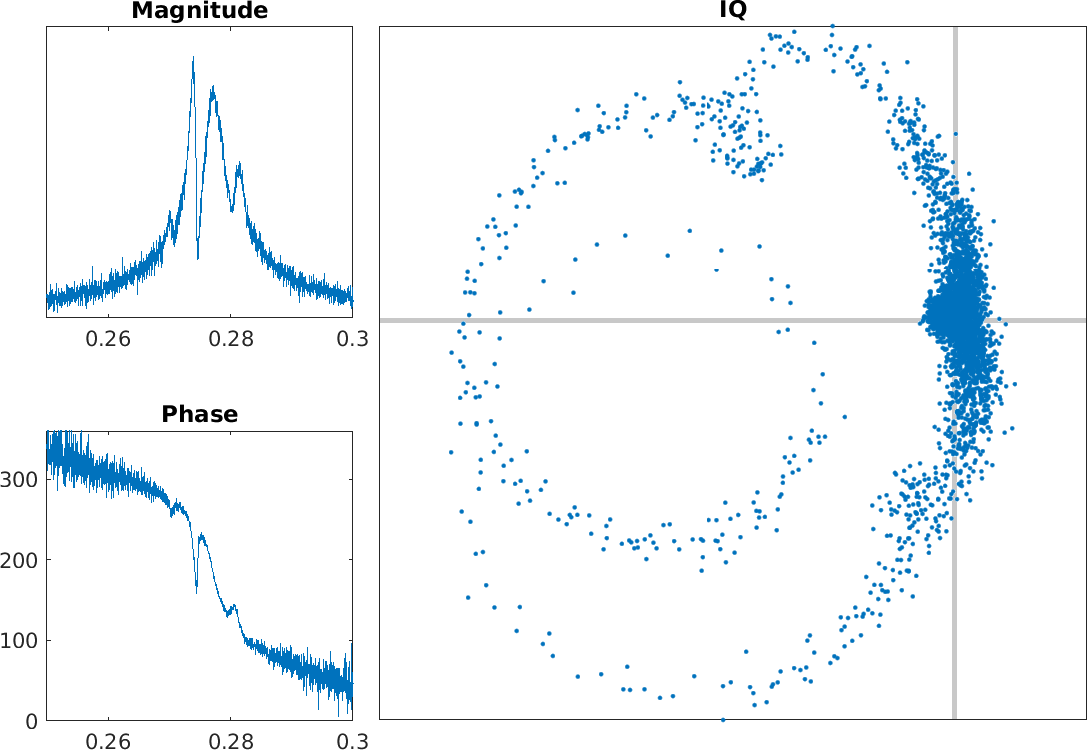
\includegraphics[width=\linewidth]{WECO03f1.png}
\squarecaption{%
Illustration of swept response, showing magnitude (in arbitrary units) and phase
(in degrees) against fractional tune, and the corresponding complex IQ
measurements.  This sweep shows a typically complex response with multiple
lobes, illustrating the problem of identifying the true tune in the presence of
large synchrotron side-lobes.
}
\label{fig:response}
\end{figure}


\section{Response Measurement}

Tune measurement at Diamond is integrated into the operation of the Multi-Bunch
Feedback (MBF) system~\cite{icalepcs2017}, and is done by exciting the beam with
a swept sinusoidal oscillation and synchronously measuring the response.  The
result is a complex number $z(\omega)$ at each sampled frequency $\omega$
representing the phase and magnitude of the machine response, computed thus:
\[
    z(\omega) = \sum_{t\in\text{dwell}(\omega)} e^{-iK\omega t} x(t)
\]
where $\text{dwell}(\omega)$ is typically 100 turns per frequency step, and $K$
is a frequency scaling factor.

Because measurement and stimulus are both confined to a single location in the
machine, we are only able to see the fractional part of the machine tune, but in
practice this is the only part that needs to be measured.  For convenience, all
frequencies $\omega$ are scaled to fractions of machine revolution frequency.

When using the MBF system for tune sweeping we have a number of options,
including which bunches to excite and measure, which overall phase advance
between bunches to apply (this is referred to as the ``mode''), strength of
excitation, and the dwell time at each frequency.  At present we excite and
measure all bunches at a mode of 80, and typically sweep 4096 points of a
frequency range of 0.1 around the nominal tune point over a period of about
780\,ms.  From this the tune measurement is updated at just over 1\,Hz.

A typical measurement is shown in Fig.~\ref{fig:response}.

\section{Modelling Measured Response}

The swept response is modelled by fitting a simple multi-pole resonator model.
Starting with the motivating example of a single narrow band resonator, this can
be described by the following differential equation (with driving term $y$,
resonator bandwidth $\nu$, nominal centre frequency $\omega_0$):
\[
    y = \ddot x + 2\nu\dot x + \omega_0^2 x \;.
\]

The Laplace transform of this gives us the following equation (where $X$, $Y$
are the Laplace transforms of $x$, $y$, and defining
$\omega_c^2\equiv\omega_0^2-\nu^2$):
\[
    Y = (s^2 + 2\nu s + \omega_0^2)X = ((s + \nu)^2 + \omega_c^2)X \;.
\]
Noting now that the quadratic term in $s$ has zeros at $s=-\nu\pm i\omega_c$,
the corresponding system response $X/Y$ can be written as (writing
$a_0\equiv1/2i\omega_c$, $b_0\equiv-\nu+i\omega_c$):
\[
    \frac XY =
    \frac{1}{(s-b_0)(s-b_0^*)} = \frac{a_0}{s-b_0} - \frac{a_0}{s-b_0^*} \;.
\]

At this point we can make some simplifying assumptions: the measured swept
response covers a narrow range around $\omega_c$, and ${\nu\ll\omega_c}$ (i.e.,
our Q factor is large).  In this case we can ignore the $a_0/(s-b_0^*)$ term and
write our model $M$ as:
\[
    M(\omega) = \frac XY(i\omega) \approx
    \frac{a_0}{i\omega-b_0} =
    \frac{a}{\omega-b}
\]
where $a\equiv-ia_0$ and $b\equiv-ib=\omega_c+i\nu$.  We work with this latter
form, which we now regard as a ``single pole resonator'', and we allow $a$ to be
a free parameter to represent other sources of scaling and phase variation which
we will want to capture.

Ignoring the small offset between damped frequency $\omega_c$ and nominal
frequency $\omega_0$, the following parameters can be computed from a single
pole $(a,b)$:
\begin{Itemize}
\item centre frequency $=\Re(b)$
\item peak width $=\Im(b)$
\item peak ``power'' $\int_\R|M(\omega)|^2d\omega=|a|^2/\Im(b)$
\item phase $=\angle i a$
\end{Itemize}

Note that the peak area $\int_\R|M(\omega)|d\omega$ diverges, and the ``power''
(integral of magnitude squared) above is a purely formal quantity, in particular
peak powers cannot meaningfully be added together.

Finally we model the full multi-pole resonator model as a sum of $N$ single pole
resonators $(a_n,b_n)_{n\in1\dotdot N}$, plus a correction factor $c$ to capture
any background offset:
\[
    M(\omega) = \sum_{n=1}^N \frac{a_n}{\omega-b_n} + c \;.
\]
This is a rational function in $\omega$, which is a natural class of functions
in control theory, and this simple model turns out to be a remarkably good fit
to measured tune sweeps.


\section{Peak Fitting Algorithm}

The input to the tune fitting algorithm is a pair of equal sized waveforms
$(\vec{\omega},\vec{z})$, where $\vec{\omega}$ is the swept frequency scale and
$\vec{z}$ is the
measured frequency response for each corresponding frequency as a complex
number.

One peak at a time is fitted to the measured data until a fitting step fails, or
until a configured number of peaks has been reached.  The peak fitting algorithm
consists of the following steps:
\begin{Enumerate}
\item Set initial model $M:=M_0$ with $N=0$, $c=0$.
\item Compute residue $\vec{r}=\vec{z}-M(\vec{\omega})$.
\item Find largest peak in $|\vec{r}|^2$ after smoothing, find region around
    this peak.
\item Compute an initial $(a,b)$ fit to $\vec{r}$ around discovered peak and
    extend model with $M'=M+(a,b)$.
\item Compute refined model $M''$ from initial model $M'$ using
    Levenberg-Marquardt optimisation
\item Assess $M''$:
    \begin{Itemize}
    \item If $M''$ fails assessment then exit with current model $M$.
    \item If $N+1=N_{\text{max}}$ then exit with new model $M''$.
    \item Otherwise assign $M:=M''$, increment $N$, go back to step 2.
    \end{Itemize}
\end{Enumerate}

At this point the peaks from the successful model are sorted into ascending
order of centre frequency and are handed over to the final tune computation
stage.


\subsection{Peak Discovery and Initial Fit}

\begin{figure}[b]
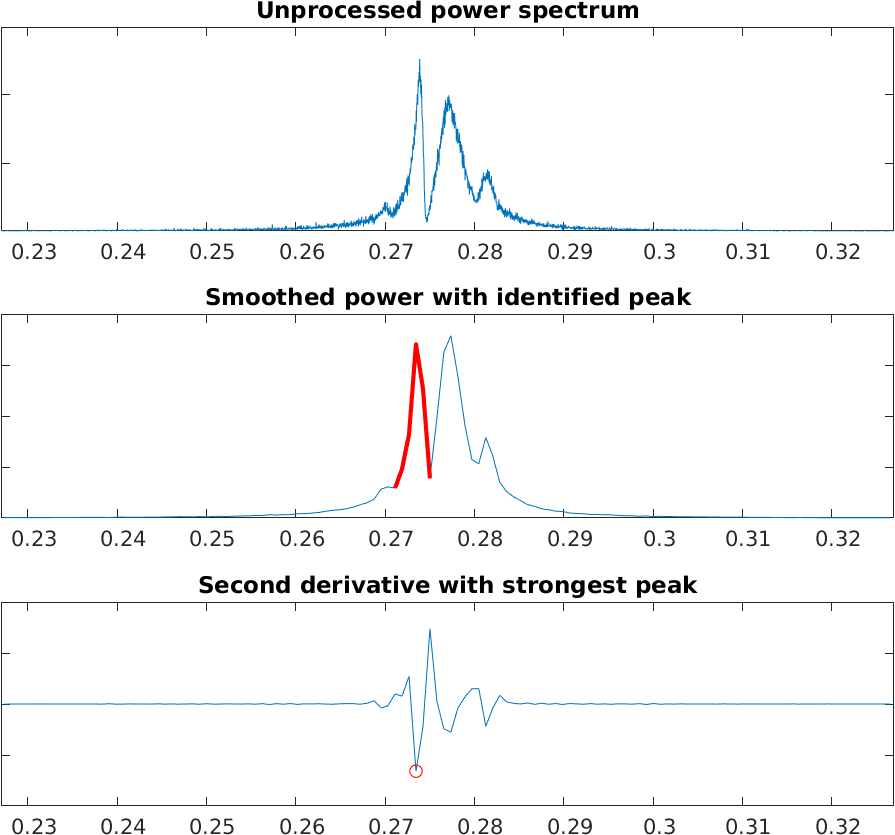
\includegraphics[width=\linewidth]{WECO03f2.png}
\squarecaption{%
Initial peak discovery: the power spectrum is smoothed and decimated, and the
strongest peak is identified by finding the frequency with the strongest
curvature (shown circled in red at bottom).  This is then used to find
the range for the initial fit (highlighted in red in the centre graph).
}
\label{fig:find-peak}
\end{figure}

Figure~\ref{fig:find-peak} shows the initial step of peak discovery.
The residue $\vec{r}$ is smoothed and decimated (we simply average in bins of 32
samples), the second derivative is computed, and the most negative point (point
of strongest curvature) is taken as the centre of the next peak to be fitted.
This starting point is then used to discover an interval $I$ spanning the
discovered peak.

Next it is important to create an initial fit to this peak to properly prime the
refinement step.  We would like to minimise the error term
$\sum_{i\in I}|r_i-a/(\omega_i-b)|^2$ over the interval $I$, but this is a
non-linear problem.  Multiplying through by $\vec\omega-b$ and a weighting term
$\vec w$ we get the minimisation problem
\[
    \text{minimise}\;\sum_{i\in I} |w_i (a + b r_i - r \omega)|^2
\]
which \emph{is} linear in $a$ and $b$ and can therefore be solved directly.  We
set $w_i\equiv|r_i|^2$ to partially cancel out the change in weighting and to
improve focusing of the fit on the centre of the peak.

This newly fitted peak is added to the model, the $c$ term is recomputed, and
the model is refined with the next step.


\subsection{Levenberg-Marquardt Optimisation}

\newcommand{\LM}{\operatorname{LM}}

The Levenberg-Marquardt (LM) algorithm\cite{levenberg, marquardt, recipies} is
an iterative non-linear least squares minimisation process.  This algorithm
takes an initial starting model and refines it iteratively to reduce the fitting
error.  We run a few rounds of this algorithm after adding each new peak to
improve the fit.

The algorithm acts on the measured machine response $(\vec\omega,\vec z)$ and
parameters $\beta=((a_n,b_n)_{n\in1\dotdot N},c)$ defining the model
$M(\omega)=M(\beta;\omega)$ to be refined.  Each step of the algorithm computes
a new $\beta'=\LM(\beta;\vec\omega,\vec{z})$ to reduce the error term
\[
    \chi^2(\beta) = \sum_i \frac{|z_i-M(\beta;\omega_i)|^2}{\sigma_i^2} \;.
\]

Ideally $\sigma_i$ should be the measurement error for $\vec{z}_i$ and should be
used to guide termination of the LM process, but at present we ignore this term.
An estimate for $\sigma$ can be probably be recovered from the tails of the
swept response, but this has not yet been investigated.

Computing $\beta'$ requires the calculation of the partial derivative terms
$\partial M(\beta;\omega)/ \partial\beta$, but fortunately these are
easy to compute:
\[
    \frac{\partial M}{\partial a_n} = \frac{1}{\omega-b_n} \;,\quad
    \frac{\partial M}{\partial b_n} = \frac{a_n}{(\omega-b_n)^2} \;,\quad
    \frac{\partial M}{\partial c} = 1 \;.
\]


\begin{figure}[ht]
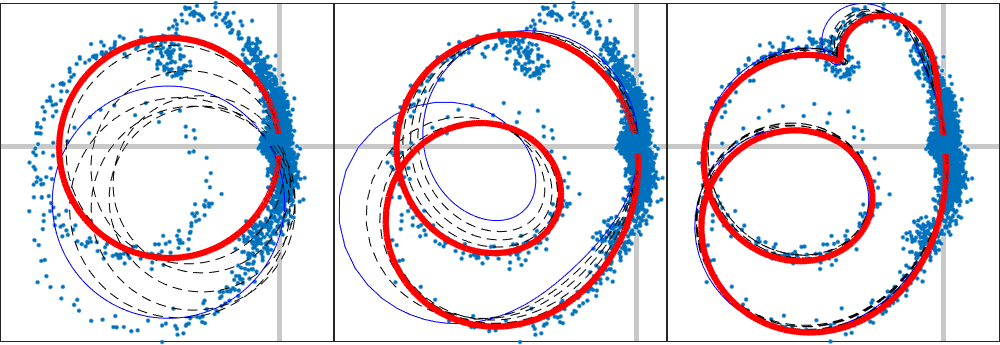
\includegraphics[width=\linewidth]{WECO03f3.png}
\squarecaption{%
Successful model refinement: fitting three poles one by one.  The red curve
shows the result after refinement, the thin blue line is the initial fit, and
the dashed lines show intermediate stages.  It is possible to see from this
figure that the first fitted pole moves from one lobe to another.
}
\label{fig:refine-ok}
\end{figure}

\begin{figure}[ht]
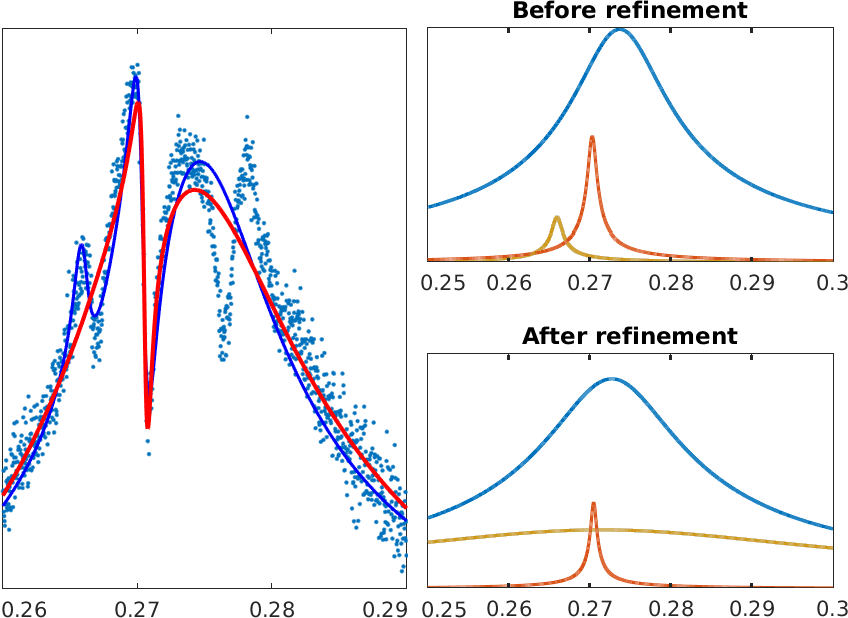
\includegraphics[width=\linewidth]{WECO03f4.png}
\squarecaption{%
Failed model refinement.  On the left the blue curve shows the initial fit, and
the top right shows the three separate components of this fit: we can see that
the small peak has been chosen.  On bottom right this peak has moved and
broadened to join the central large peak: this fit is rejected by the model
assessment step.
}
\label{fig:refine-fail}
\end{figure}


\subsubsection{Behaviour of LM Refinement}

This algorithm is very sensitive to initial conditions, and can produce some
unhelpful results: the biggest problem is a tendency for poles to wander and
interfere with one another.  This problem becomes more pronounced as more poles
are added, and in general it is difficult to fit all three peaks reliably.

Figure \ref{fig:refine-ok} shows the process of successful incremental peak
fitting and refinement.  Figure~\ref{fig:refine-fail} shows the more complex
case of failing when adding a third peak: in this case we see the importance of
the initial conditions.


\subsection{Model Assessment}

It is important to evaluate the success of the tune fitting process, so after
each LM optimisation step the entire model is assessed.  This involves the
following checks, if any of them fail the entire fit is discarded:
\begin{Itemize}
\item Peak width.  The peak width is checked against configured minimum and
    maximum limits.  This catches peaks that have run away into the background
    (very broad peaks), peaks that have got caught on local noise (very narrow
    peaks), and peaks that have gone negative.
\item Peak position.  Occasionally the centre of a peak will wander out of the
    swept data window, and so must be treated as invalid.
\item Peak closeness.  If two peaks are too close together this is a clear sign
    of peak merging, and so the model can be discarded.
\item Peak merging.  Peaks with opposing phase are also a sign of peak merging
    and cause the model to be rejected.
\end{Itemize}



\begin{figure}[ht]
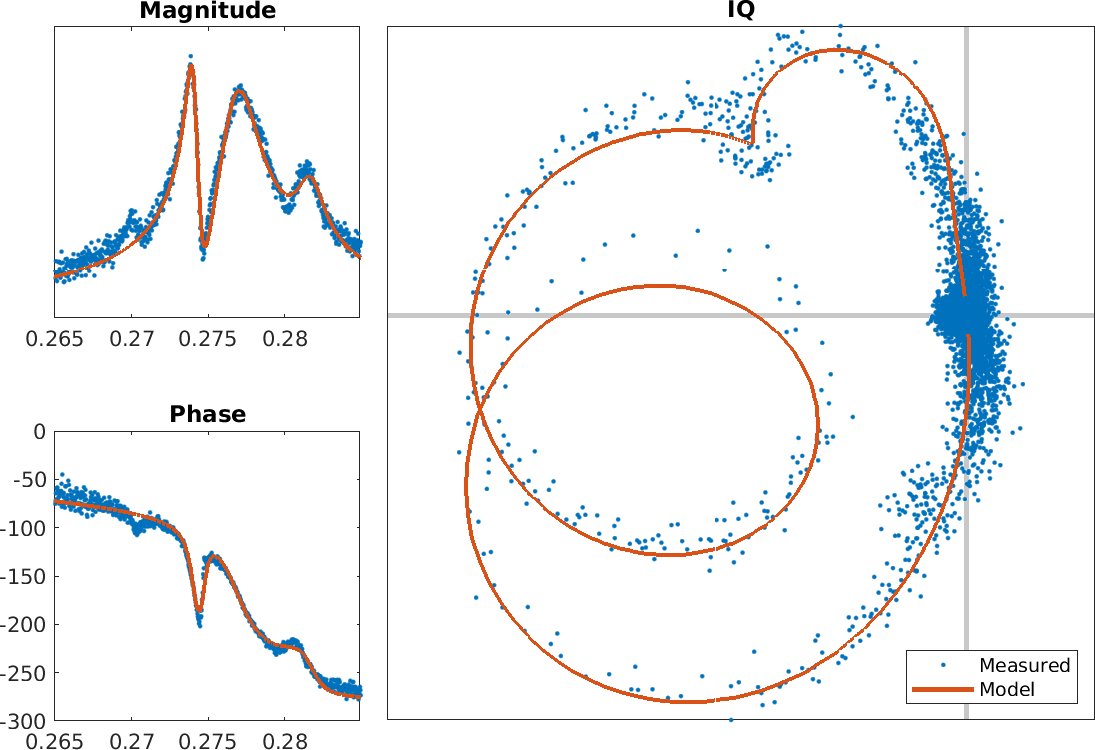
\includegraphics[width=\linewidth]{WECO03f5.png}
\squarecaption{%
This figure show a successful fit of a three pole model to a typical tune sweep.
The two main peaks are fitted very closely, the third peak looks slightly off,
while there is a fourth peak which has not been attempted.  From this model we
can measure a tune of 0.2768 with a phase of 159\textdegree{} (seen through the
MBF feedback filter).
}
\label{fig:full-fit}
\end{figure}


\subsection{Computing the Tune}

The original motivation for fitting as many peaks as possible was to find a way
to reliably identify the true ``tune''.  In practice it seems that simply taking
the peak with the largest ``power'' is sufficient.  From the model we can now
read out the tune, its phase and bandwidth or damping factor, and the
synchrotron side bands, if they were successfully fitted.

Figure~\ref{fig:full-fit} shows the final result of a successful fit to the data
captured in Fig.~\ref{fig:response} and refined in Fig.~\ref{fig:refine-ok}.


\begin{figure}[ht]
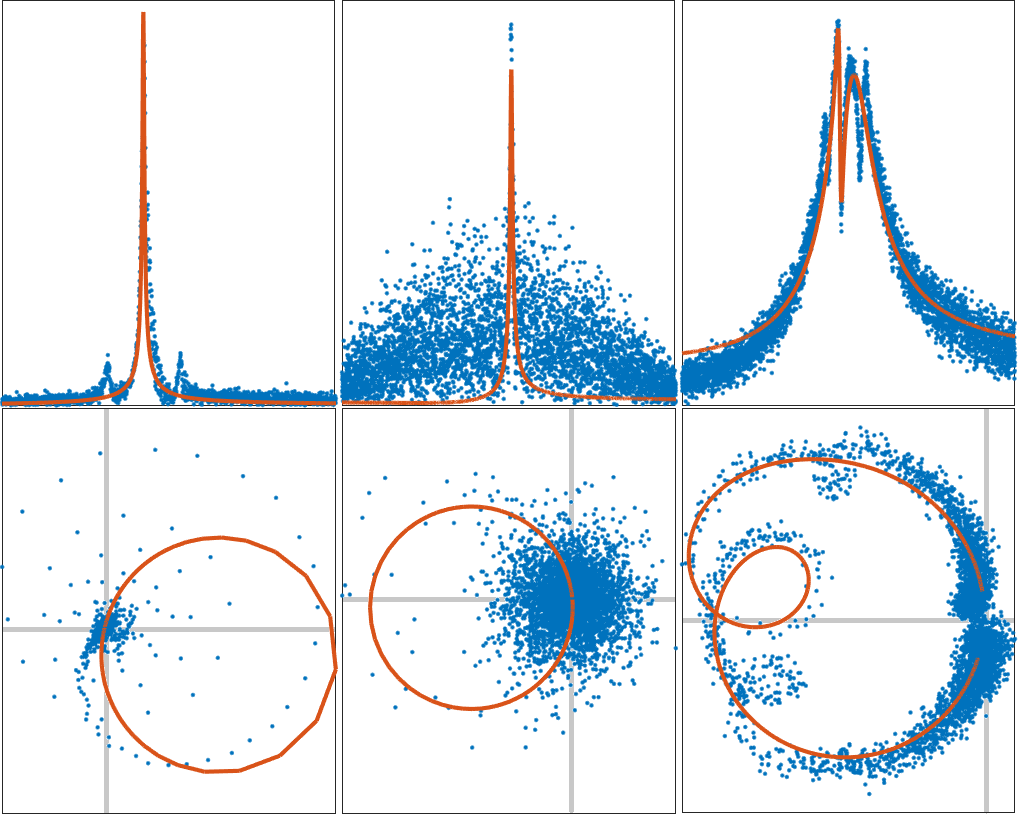
\includegraphics[width=\linewidth]{WECO03f6.png}
\squarecaption{%
Three challenging fits: magnitude and IQ shown.  The first sweep shows
strong ringing from sweeping a narrow resonance too quickly, but the fit is
successful.  The second sweep shows the limit of tune detection, but is again
successful.  The third sweep shows failure to fit the third important lobe: in
this case feedback is flattening the tune response.
}
\label{fig:challenge-zoo}
\end{figure}


\begin{figure}[ht]
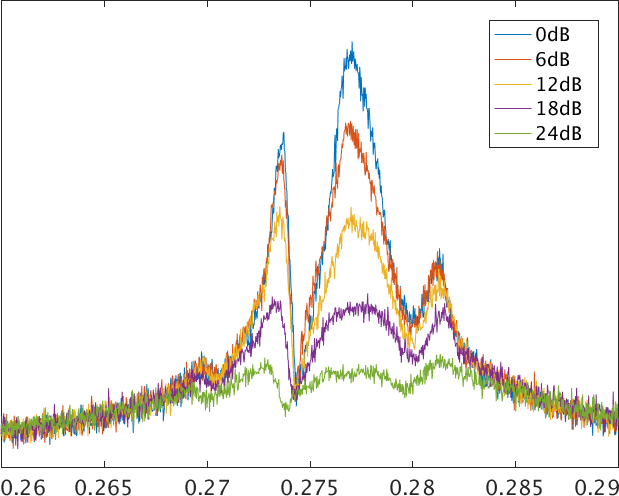
\includegraphics[width=\linewidth]{WECO03f7.png}
\squarecaption{%
Tune sweeping measurement is normally combined with bunch-by-bunch feedback.
This figure shows the impact of the feedback intensity on the tune sweep:
increasing feedback flattens the response and makes the fit less reliable.
}
\label{fig:feedback}
\end{figure}


\section{Challenges}

The main challenge has been to develop an algorithm that is robust enough to
produce acceptable results throughout the entire operating range of the
synchrotron.  In particular, tune sweeps look completely different at low and
high beam currents, and high chromaticity enhances the synchrotron sidebands.

At very low beam currents the tune resonance can become extremely narrow.  The
main impact of this is ``dragging'' of the resonance with the sweep, producing
extra oscillations on the swept response.  This can be avoided with a narrower
or slower sweep.

A small selection from some more challenging sweeps is shown in
Fig.~\ref{fig:challenge-zoo}.  In all three cases the data can be improved by
changing the sweep conditions.  Figure~\ref{fig:feedback} shows the impact of
correcting for multi-bunch instabilities on response measurement.


\section{Conclusions}

This algorithm has been developed and has evolved over many years.  Throughout
the main problem has been to distinguish the true ``tune'' peak from its
neighbours.  Now with a reasonably reliable algorithm producing a detailed and
accurate fit (when successful) we are able to measure the tune for long periods
without ``hopping'' to adjacent peaks.

Problems still remain with challenging machine conditions, particularly when
very strong bunch-by-bunch feedback is required, when operating at extremely low
beam currents, or at very high chromaticities.  However for normal operation
this algorithm is very reliable and is able to operate unattended for long
periods.

The code for the tune fitting algorithm is written in Python and can be obtained
by contacting the author.


\begin{thebibliography}{99}


\bibitem{icalepcs2017}
M.G.~Abbott, G.~Rehm, and I.S.~Uzun,
\enquote{A New Transverse and Longitudinal Bunch by Bunch Feedback Processor}
in \emph{Proc. 16th Int. Conf. on Accelerator and Large Experimental Control
Systems (ICALEPCS'17)}, Barcelona, Spain, Oct. 2017, pp. 1649--1654.
\url{doi:10.18429/JACoW-ICALEPCS2017-THPHA115}

\bibitem{levenberg}
K.~Levenberg, \enquote{A Method for the Solution of Certain Non-Linear Problems
in Least Squares}, in \emph{Quart. Appl. Math.}, vol.~2, pp.~164--168, 1944.
\url{doi:10.1090/qam/10666}

\bibitem{marquardt}
D.W.~Marquardt, \enquote{An algorithm for least-squares estimation of nonlinear
parameters}, in \emph{J. Soc. Indust. Appl. Math.}, vol.~11, no.~2,
pp.~431--441, 1963.
\url{doi:10.1137/0111030}

\bibitem{recipies}
W.H.~Press, B.P.~Flannery, S.A.~Teukolsky, W.T.~Vetterling,
\emph{Numerical Recipes in C: The Art of Scientific Computing}.
New York, NY, USA:Cambridge University Press,
1988, ch.~14, sec.~4, pp.~540--547.


\end{thebibliography}


\end{document}
